 




\documentclass[]{report}   % list options between brackets
\usepackage{graphicx}            % list packages between braces
\usepackage{amsmath}

% type user-defined commands here

\begin{document}


\title{Vaja 2: Uklon in interferenca}   % type title between braces
\author{Dominik Zagrusovcem,
Lucija grabar}
         % type author(s) between braces
\date{3.8.2024}    % type date between braces
\maketitle
\section{Diferencialna enačba}
za program sem uporabil eulerjevo metodo ker je najlažja za implementirati in ker če bi hotel biti učinkovit sploh nebi numerično reševal diferecialnih enačb ampak programsko analitično določil trajektorije.
\section{Odboj}
za delujučo simulacijo potrebujemo dobro definiran odboj.
\subsection{pogoj za odboj}
Pogoj za odboj je takrat ko je točkasto telo v polkrožni cevi.
Če definiramo koordinatno izhodišče v središču cevi lahko lahko definiramo pogoj takole.
\[(r_c^2<x^2+y^2) \implies odboj \]
ko je ta pogoj izpolnjen je pametno pozicijski vektor normirati na polmer kroga da ni možnkosti,da bi se delec zagozdil zunaj defineiranega območja
\[
\vec{r}_{new}=r_{max}\frac{\vec{r}_{old}}{|\vec{r}_{old}|}
\]

\subsection{odboj}
Če zanemarimo trenje je lahko odbojna sila le radialna. Potemtakem lahko definiramo odboj kot obrat radialne sile.
Da to storimo, moramo seveda najprej projecirati vektor hitrosti na radialni enotski vektor in pomnožiti z dva.
\[
c = \frac{\vec{v} * \vec{r}}{|\vec{r}|}
\]
\[
\vec{v}_{new}= \vec{v}_{old}-2\frac{\vec{r}}{|\vec{r}|}c
\]
Ob vsakem odboju se tudi ostane le 90\% energije iz tega lahko izpeljemo faktor zmanjšanja hitrosti.
\[
\frac{(v_{new}^2)}{v_{old}^2}=0.9 \implies \vec{v}_{new}=\vec{v}_{old} \sqrt{0.9}
\]
\section{Analiza napak}
Eulerjeva metoda ustvarja napake. najlažji način prikazovanja tega je skupna mehanska energija ($E$) ki bi se morala ohranjati pri prostem padu. za analizo napake sem uporabil začetni primer $\vec{r}=(0,0.1),\vec{v}=(0,0)$ \newpage

\begin{figure}[h!]
    \centering
    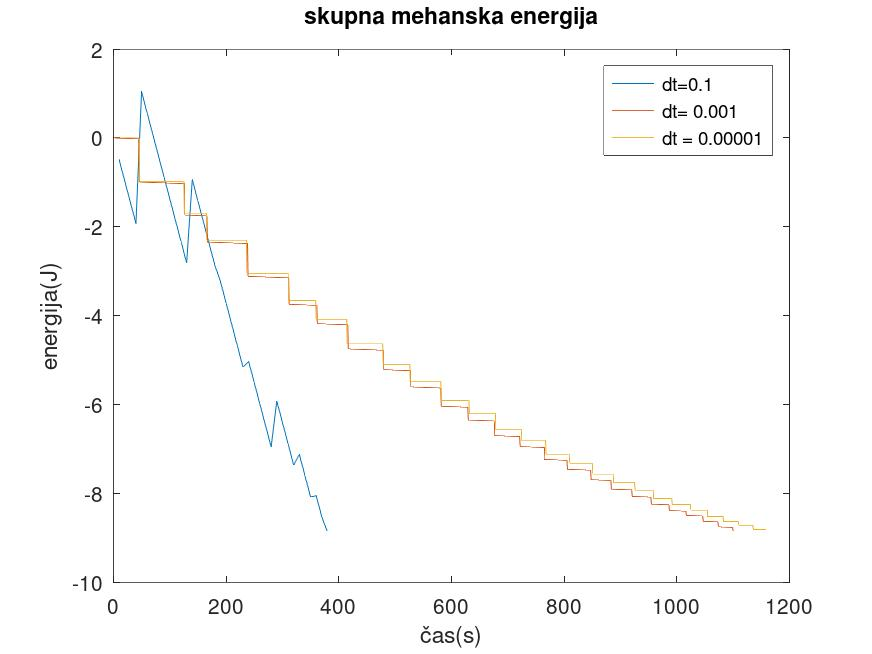
\includegraphics[width=0.8\textwidth]{errorE.jpg} % Path to the image
    \caption{graf skupne mehanske energije pri različnih dt}
    \label{fig:scatter_plot}
\end{figure}
Na grafu pričakujemo ravne črte in diskretne padce v energiji ob odbojih. 
Iz grafa se je očitno razvidno, da simulacija pri velikih časovnih korakih preide v čisto nefizikalen režim
(energija se niti približno ne ohranja in ob odboju se celo poveča). pri majhnih časovnih korakih pa se približno ohranna in vidimo pojave ki bi jih pričakovali.
\subsection{zanimivost}
pri reševanju takšnih diferencialni enačb je vrstni red operacij zelo pomemben, saj če eno vrednost posodobimo za ali pred drugo lahko precej spremenimo stabilnost programa.
\begin{figure}[h!]
    \centering
    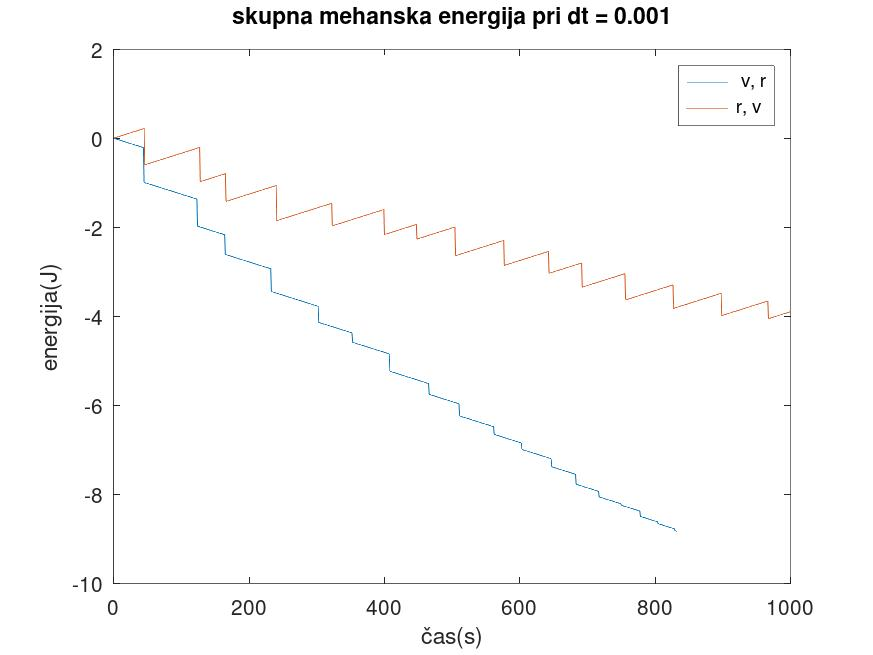
\includegraphics[width=0.8\textwidth]{errorEcring2.jpg} % Path to the image
    \caption{graf skupne mehanske energije pri razlih metodah ko je dt =0.01}
    \label{fig:scatter_plot}
\end{figure}
če  najprej posodobimo $\vec{v}$  numerična napaka povzroči večanje skupne energije s časaom. Če pa najprej posodobimo $\vec{r}$ pa povzroči padanje energije. 

\begin{figure}[h!]
    \centering
    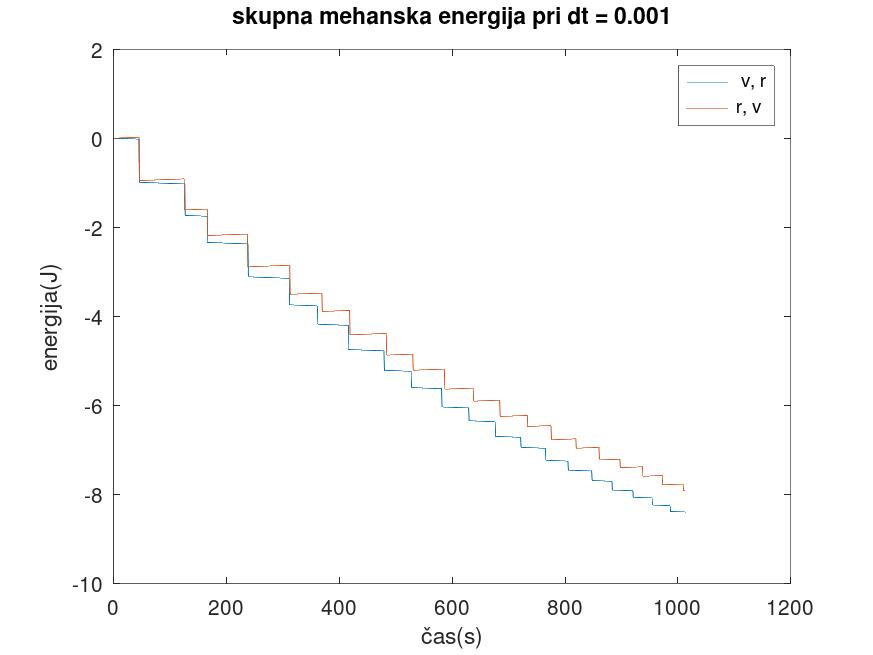
\includegraphics[width=0.8\textwidth]{errorEcring.jpg} % Path to the image
    \caption{graf skupne mehanske energije pri razlih metodah ko je dt =0.001}
    \label{fig:scatter_plot}
\end{figure}
Pri manjših časovnih korakih pa rešitve konvergirajo skupaj

\end{document}
\\